\section{Conceitos}

\begin{frame}{Conceitos - Fatores que influenciam a AA}

\begin{columns}
	\begin{column}{0.48\textwidth}
		\begin{tcolorbox}[title=Canal,height=2.4cm,valign=center]
			E-mail, jornais, livros, SMS
			\tcblower
			Textos mais ou menos formais.                    
		\end{tcolorbox}
	\end{column}
	\begin{column}{0.48\textwidth}
		\begin{tcolorbox}[title=Idioma,height=2.4cm,valign=center]
			Complexidade morfológica e lexical diferentes.
		\end{tcolorbox}
	\end{column}
\end{columns}
\begin{columns}
	\begin{column}{0.48\textwidth}
		\begin{tcolorbox}[title=Tópico,height=2.4cm,valign=center]
			Economia, celebridades, dia-a-dia
			\tcblower
			Influencia o vocabulário.                    
		\end{tcolorbox}
	\end{column}
	\begin{column}{0.48\textwidth}
		\begin{tcolorbox}[title=Domínio ou Gênero do texto,height=2.4cm,valign=center]
			Contos, romances, artigos
			\tcblower
			Influencia no rigor formal e no vocabulário.
		\end{tcolorbox}
	\end{column}
\end{columns}

\begin{columns}
	\begin{column}{0.48\textwidth}
	\begin{tcolorbox}[title=Tamanho do texto,height=2.4cm,valign=center]
		Métodos probabilísticos são afetados pelo número de observações. formais.                    
	\end{tcolorbox}
	\end{column}
	\begin{column}{0.48\textwidth}
	\begin{tcolorbox}[title=Número de autores,height=2.4cm,valign=center]
	O aumento do número de classes requer o aumento do número de classes.                    
	\end{tcolorbox}
	\end{column}
\end{columns}

\end{frame}






%%%%%%%%%%%%%%%%%%%%%%%%%%%%%%%%%%%%%%%%%%%%%%%%%%%%%%%
\begin{frame}{Conceitos - Subtarefas da análise autoral}
\begin{columns}
	\begin{column}{0.48\textwidth}
		\begin{tcolorbox}[colback=red!5!white,colframe=red!75!black,title=AA de conjunto fechado,height=2.4cm,valign=center]
			Os textos do conjunto de teste pertencem a um dos autores candidatos presentes no córpus de treinamento.                    
		\end{tcolorbox}
	\end{column}
	\begin{column}{0.48\textwidth}
		\begin{tcolorbox}[title=AA de conjunto aberto,height=2.4cm,valign=center]
			Os textos do conjunto de teste não necessariamente foram escritos por um dos autores do córpus de treinamento                    
		\end{tcolorbox}
	\end{column}
\end{columns}

\begin{columns}
	\begin{column}{0.48\textwidth}
		\begin{tcolorbox}[title=K-Atribuição ou ordenação ,height=2.4cm,valign=center]
			As saídas do classificador são ordenadas pela probabilidade e são retornados os K autores mais prováveis.
		\end{tcolorbox}
	\end{column}
	\begin{column}{0.48\textwidth}
		\begin{tcolorbox}[title=Caracterização,height=2.4cm,valign=center]
			São extraídas informações demográficas do autor do texto podem reduzir a lista de candidatos.                    
		\end{tcolorbox}
	\end{column}
\end{columns}

\begin{columns}
	\begin{column}{0.48\textwidth}
		\begin{tcolorbox}[colback=green!5!white,colframe=green!75!black,title=Verificação,height=2.4cm,valign=center]
			Verifica-se se dois documentos foram escritos pelo mesmo autor, não sendo necessário saber quem são os autores.                
		\end{tcolorbox}
	\end{column}
	\begin{column}{0.48\textwidth}
		\begin{tcolorbox}[title=Demais,height=2.4cm,valign=center]
			Agrupamento, Ligação e Quebra de estilo.                    
		\end{tcolorbox}
	\end{column}
\end{columns}

\end{frame}

%%%%%%%%%%%%%%%%%%%%%%%%%%%%%%%%%%%%%%%%%%%%%%%%%%%%%%%
\begin{frame}{Conceitos - Tipos de conhecimentos usados}

A abordagem estilométrica tradicional utiliza as seguintes fontes de conhecimento:

\begin{itemize}
	\item {\bf Categoria lexical:} tamanho médio das palavras, número de letras maiúsculas, tamanho das sentenças, etc.
	
	\item {\bf Categoria sintática:} frequência da pontuação, palavras de função, etc.
	
	\item {\bf Categoria semântica:} contagem das palavras, analisadores semânticos, {\it word embeddings}, etc. 
	
	\item {\bf Categoria específica de domínio:} palavras-chave, {\it tags} HTML, {\it emoticons}, etc.
\end{itemize}
\end{frame}

%%%%%%%%%%%%%%%%%%%%%%%%%%%%%%%%%%%%%%%%%%%%%%%%%%%%%%%
\begin{frame}{Conceitos - Tipos de conhecimentos usados}
	\begin{tcolorbox}[colback=blue!1!white,colframe=blue!35!black,title=Palavras,height=3cm,valign=center]
		As palavras mais frequentes de um texto são independentes de domínio e utilizadas de forma inconsciente \cite{Kestemont2014}.\\ \\
		{\bf Palavras de função} (do inglês, {\it function words}) compreende artigos, preposições, locuções adverbiais, e outros.	
	\end{tcolorbox}

	\begin{tcolorbox}[colback=green!1!white,colframe=green!35!black,title=Caracteres,height=4cm,valign=center]
		As sequências de caracteres são considerados os modelos mais efetivos para AA \cite{KjellWF94,Neal2017} e uma contagem simples pode produzir modelos próximos ao estado-da-arte \cite{Neal2017}.\\ \\
		Os {\bf caracteres mais frequentes (CNG)} (do inglês, {\it common n-grams}) \cite{Keselj2003,Sapkota2014}.
	\end{tcolorbox}
\end{frame}

%%%%%%%%%%%%%%%%%%%%%%%%%%%%%%%%%%%%%%%%%%%%%%%%%%%%%%%
\begin{frame}{Conceitos - Modelos computacionais}
\begin{tcolorbox}[title=Modelo tradicional de representação textual,valign=center]
	\begin{itemize}
		\item Hipótese distribucional aplicada à documentos \cite{Turney2010}
		\item N-gramas
		\item Conhecimentos: Caractere, Palavras, POS
		\item TF-IDF
		\item TF-IDF equações alternativas utilizadas nos experimentos:
			\begin{itemize}
				\item $ TF_{sublinear} = 1 + \log TF_{t,d}$ 
				\item $
				IDF_{Suavizado}(t,D) = log\left (
				\frac{D}{DF(t)}
				\right ) + 1
				$
			\end{itemize}
	\end{itemize}	
\end{tcolorbox}
\end{frame}


\begin{frame}{Conceitos - Modelos computacionais}

\begin{columns}
	\begin{column}{0.60\textwidth}\selectFont
		\begin{tcolorbox}[title=Modelo de representação distribuída,valign=center]
			\begin{itemize}
				\item Hipótese distribucional aplicada símbolos
				\item Modelos neurais de língua natural \cite{Bengio2003}
				\item {\it Word embeddings} 
				\begin{itemize}\selectFont
					\item Representa cada palavra, ou símbolo, em k dimensões, sendo k menor que o tamanho do vocabulário.
					\item Word2Vec \cite{Mikolov2013}
					\item Doc2Vec \cite{QuocLe2014}
					\item FastText 
				\end{itemize}
			\end{itemize}
		\end{tcolorbox}
	\end{column}
	\begin{column}{0.40\textwidth}
		\begin{tcolorbox}[title=Modelo Word2Vec,valign=center]
		   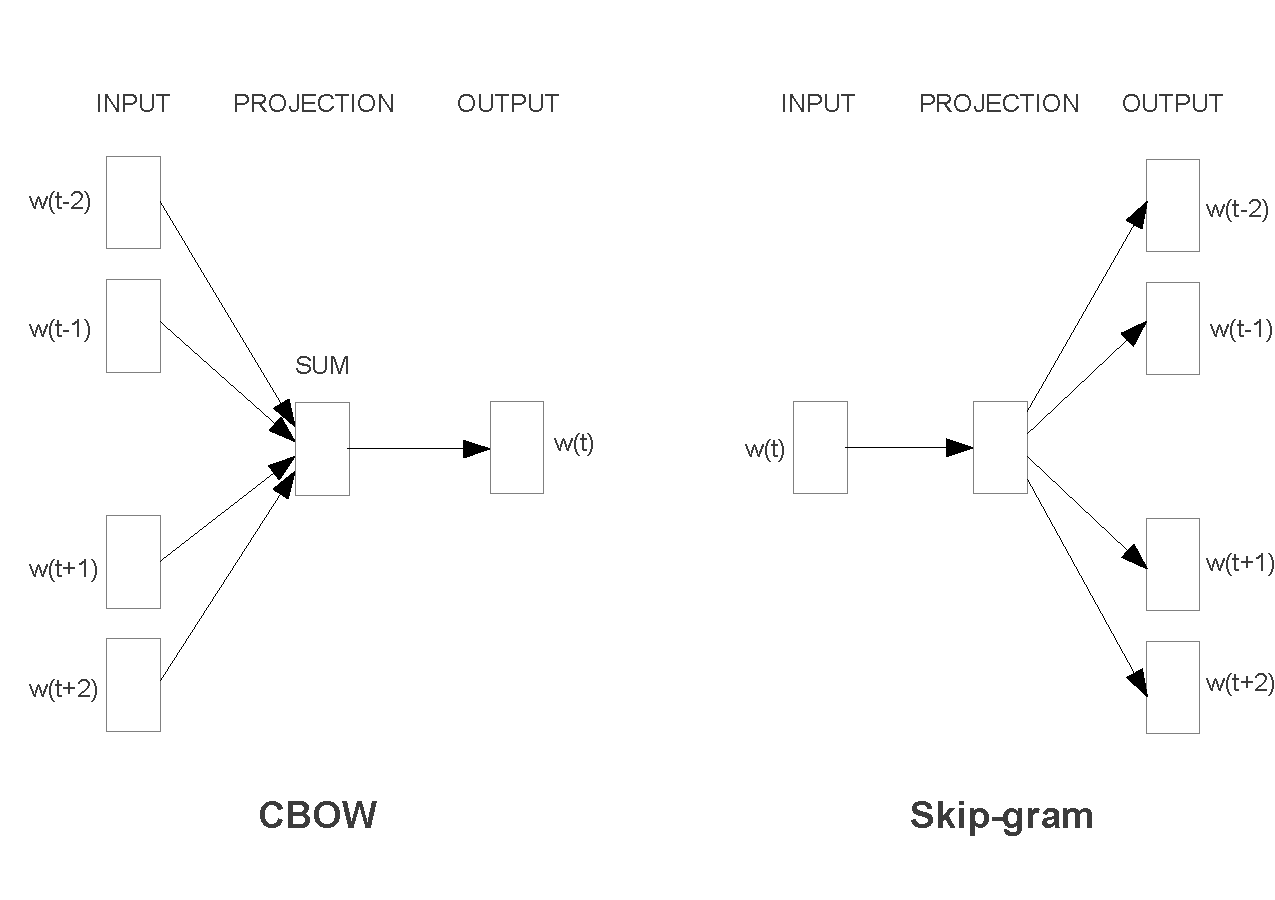
\includegraphics[width=.99\textwidth]{images/efficient-models.pdf}
		\end{tcolorbox}
	\end{column}
\end{columns}

\end{frame}
